\documentclass[onecolumn, oneside, letterpaper, draftclsnofoot, 10pt, compsoc]{IEEEtran}

\usepackage[english]{babel}
\usepackage{graphicx}
\usepackage{url}
\usepackage{setspace}
\usepackage{subcaption}
\usepackage{verbatim}
\usepackage{amssymb}
\usepackage{amsmath}
\usepackage{amsthm}
\usepackage{alltt}
\usepackage{color}
\usepackage{enumitem}
\usepackage{textcomp}
\usepackage{cite}
\usepackage{float}

%\usepackage[T1]{fontenc}
\usepackage[utf8]{inputenc}
\usepackage{lmodern}
\usepackage[hidelinks]{hyperref}
\usepackage[normalem]{ulem}

\usepackage[margin=0.75in]{geometry}

%\parindent = 0.0 in
%\parskip = 0.05 in

% 1. Fill in these details
\def \CapstoneTeamName{         Beaver Hawks}
\def \CapstoneTeamNumber{       14}
\def \GroupMemberOne{           Anton Synytsia}
\def \GroupMemberTwo{           Matthew Phillips}
\def \GroupMemberThree{         Shanmukh Challa}
\def \GroupMemberFour{          Nathan Tan}
\def \CapstoneProjectName{      American Helicopter Society Micro Air Vehicle Competition}
\def \CapstoneSponsorCompany{   Potentially Columbia Helicopters}
\def \CapstoneSponsorPerson{    Nancy Squires}

% 2. Uncomment the appropriate line below so that the document type works
\def \DocType{Winter Progress Report}

\newcommand{\NameSigPair}[1]{\par
\makebox[2.75in][r]{#1} \hfil   \makebox[3.25in]{\makebox[2.25in]{\hrulefill} \hfill        \makebox[.75in]{\hrulefill}}
\par\vspace{-12pt} \textit{\tiny\noindent
\makebox[2.75in]{} \hfil        \makebox[3.25in]{\makebox[2.25in][r]{Signature} \hfill  \makebox[.75in][r]{Date}}}}
% 3. If the document is not to be signed, uncomment the RENEWcommand below
%\renewcommand{\NameSigPair}[1]{#1}

%%%%%%%%%%%%%%%%%%%%%%%%%%%%%%%%%%%%%%%
\begin{document}
\begin{titlepage}
    \pagenumbering{gobble}
    \begin{singlespace}
        %\includegraphics[height=4cm]{coe_v_spot1}
        \hfill
        % 4. If you have a logo, use this includegraphics command to put it on the coversheet.
        \begin{center}
        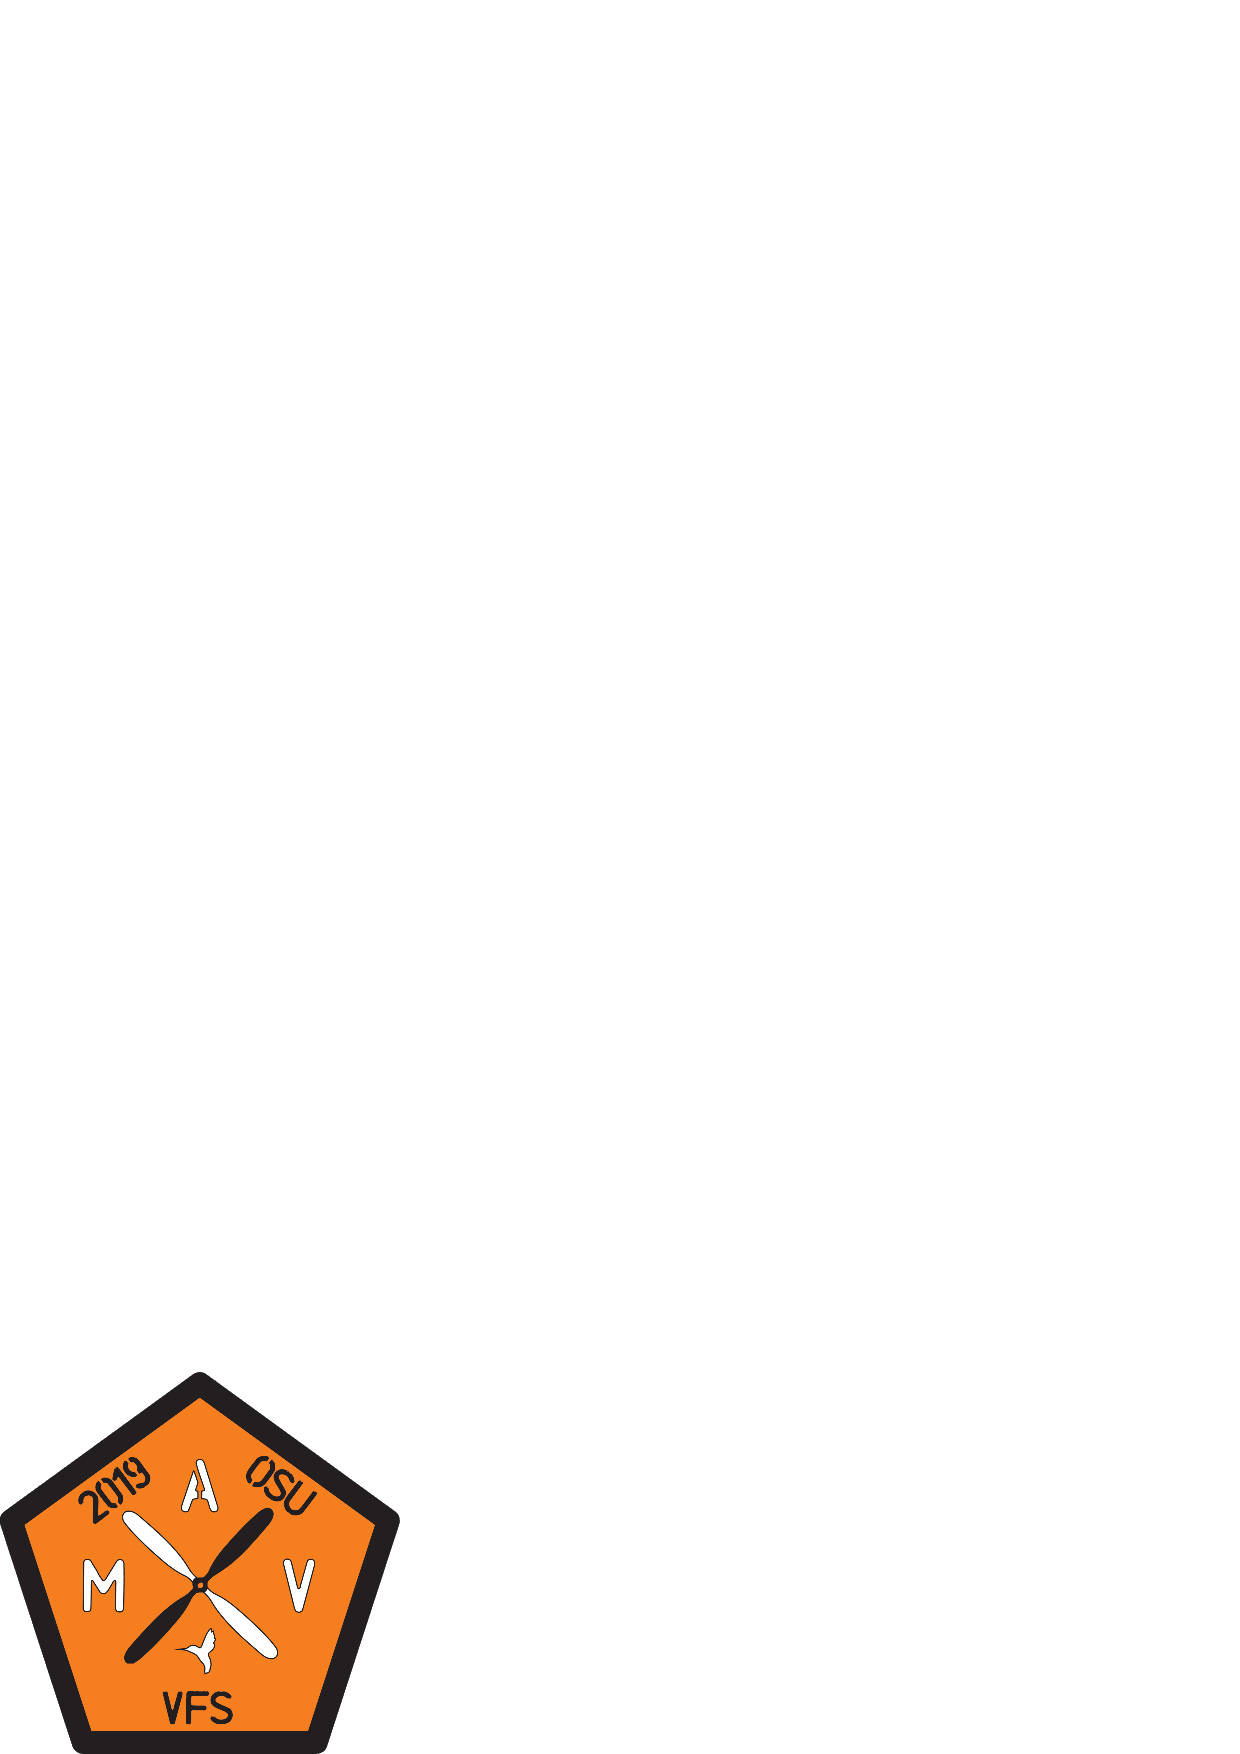
\includegraphics[height=4cm]{graphics/logo.png}
        \end{center}
        \par\vspace{.2in}
        \centering
        \scshape{
            \huge CS Capstone \DocType \par
            {\large\today}\par
            \vspace{.5in}
            \textbf{\Huge\CapstoneProjectName}\par
            \vfill
            {\large Prepared for}\par
            \Huge \CapstoneSponsorCompany\par
            \vspace{5pt}
            {\Large\NameSigPair{\CapstoneSponsorPerson}\par}
            {\large Prepared by }\par
            Group\CapstoneTeamNumber\par
            % 5. comment out the line below this one if you do not wish to name your team
            \CapstoneTeamName\par
            \vspace{5pt}
            {\Large
                \NameSigPair{\GroupMemberOne}\par
                \NameSigPair{\GroupMemberTwo}\par
                \NameSigPair{\GroupMemberThree}\par
                \NameSigPair{\GroupMemberFour}\par
            }
            \vspace{20pt}
        }
        \begin{abstract}
        \end{abstract}
    \end{singlespace}
\end{titlepage}
\newpage
\pagenumbering{arabic}
\tableofcontents
% 7. uncomment this (if applicable). Consider adding a page break.
\listoffigures
%\listoftables
\clearpage

\section{Project Purpose and Goals}
The Vertical Flight Society (VFS) is the world\textquotesingle s premiere international technical society for engineers, scientists and others working to advance vertical flight. VFS brings together industry, academia and government to face difficult challenges in vertical flight. Each year, VFS hosts the Micro Air Vehicle challenge to help prepare and attract the next generation of scientist and engineers to work in the field of vertical flight.

\noindent
\newline
The goal of this project is to collaborate closely with the mechanical engineering and electrical engineering subteams in building a micro air vehicle to accomplish the mission presented by the Vertical Flight Society.


\section{Current Progress}
\subsection{Overview}
Our team has been meeting consistently throughout the term and are making great progress in completing the project. While the Electrical Engineering team was installing the devices on the helicopter, the computer science team began by developing a web application with placeholders for specific data feeds such as front-facing camera, bottom-facing camera, depth map, attitude, and sensor data.

\noindent
\newline
Currently, most of our core functionality is available on our user interface. The Electrical Engineering team has installed our bottom facing camera and we are able to display live video feeds through our application.

\noindent
\newline
The helicopter has gone through a couple iterations on its frame, but now it has been altered into a triangular prism shape to help reduce the weight (as shown in figure ). As far as the way this affects the CS team, our only big concern is the angling of the ultrasonic sensors for our calculations if we reach our stretch goal of implementing collision avoidance.

\begin{figure}[H]
    \centering
    \includegraphics{graphics/Helicopter.PNG}
    \caption{Helicopter Body}
    \label{fig:heli}
\end{figure}

\subsection{Design Summary}
% Anton
\noindent
Reflecting on the design, we have a significant portion of the user interface completed. We initially setup a NodeJS server for the user interface. The server is a prerequisite for all the design requirements. We then created a very low fidelity prototype for the main page, consisting of HTML and CSS. Having the layout, we then focused on developing GUI elements for the flight instruments, porting the camera feed, generating random values, creating a data recording mechanism, and developing a portion of the code on the Raspberry Pi.

\subsection{Collision Warning GUI}
% Anton
\noindent
There are two flight instruments that involve GUI. They are collision warning and attitude indicator. For the alpha version, we have only implemented the collision warning instrument. The collision warning instrument displays three sensor ranges in a color-coded format. The floating point sensor ranges, which range from 6 to 254 inches, are converted to their appropriate colors and applied to their associated collision warning GUI elements. The colors transition from green being the farthest, to yellow being the intermediate, to red being the closest, with example states displayed in figures \ref{fig:cw1}, \ref{fig:cw2}, and \ref{fig:cw3}. At the moment, the three ranges are fed in by our transitioning random value generator. The transitioning value generator, which we have also developed, provides the functionality for testing our implementation until we obtain feed from the actual sensors.
%\iffalse
\begin{figure}[!htb]
\minipage{0.32\textwidth}
  \includegraphics[width=\linewidth]{graphics/collision_warning1.png}
  \caption{Collision Warning A}
  \label{fig:cw1}
\endminipage\hfill
\minipage{0.32\textwidth}
  \includegraphics[width=\linewidth]{graphics/collision_warning2.png}
  \caption{Collision Warning B}
  \label{fig:cw2}
\endminipage\hfill
\minipage{0.32\textwidth}%
  \includegraphics[width=\linewidth]{graphics/collision_warning3.png}
  \caption{Collision Warning C}
  \label{fig:cw3}
\endminipage
\end{figure}
%\fi

\subsection{Wifi Data Transmitter}
% Anton
\noindent
Speaking of sensor feed, we developed a wireless data transmitter to communicate information between the Raspberry Pi and the server. Our wirelesss data transmitter is based on the User Datagram Protocol (UDP) and Transmission Control Protocol (TCP). UDP is used for sending non-important, although useful, bits of information from the Raspbian, which is based on the the Raspberry Pi, and to the server, which is based on one the laptops. The non-important bits include all the ultrasonic sensor data and gyroscope angles. TCP, on the other hand, is used for transmitting important bits, such as for manipulating the controls on the Micro Air Vehicle (MAV).

% Anton
\noindent \\
Getting into the details of our wireless data transmitter, the way it works is that the IP addresses, for transmitting the packets across, are not hard-coded. We actually developed a functionality that allows the server and the Raspberry Pi to familiarize with each others IP addresses. When the server is started, it multi-casts a signal to a specific multi-cast address and port. At the same time, the server also starts a listener coming to any of its interfaces at the pre-defined port. When the Raspberry Pi is turned on, a boot-up script launches a multi-cast receiver, which listens for the messages coming to the pre-defined multi-cast address and port. Upon receiving a signal at the pre-defined multi-cast port and address, the Raspberry Pi extract the IP address of the interface that sent the packet, which presumably is the IP address of the server, and then sends a response to the extracted IP address, at a pre-defined port number. Upon receiving a response at the pre-defined, the server extracts the sender IP address, which is presumably the IP address of the Raspberry Pi, and establishes an IP-based communication, for sending data back and forth. When we say, ``presumably'', we actually have two, predefined messages: ``BeaverHawks-1'' and ``BeaverHawks-2'', that we check the received messages against, just as a weak barrier against a potential hacker. We call the set of steps for identifying the IP addresses a handshake and for the handshake we use UDP. This all works provided the Raspberry Pi and the server are connected to the same Wifi network.

% Anton
\noindent \\
Speaking of networks, the school\textquotesingle s routers block our multi-cast signals, even though we are able to connect both, the server and the Raspberry Pi, to the same Wifi network. For that reason, and for portability, in general, we decided to get a router and a wireless access point. We will configure the router to permit multi-cast signals, for the compatibility of our handshake system. And just to mention, up until now, we tested our data transmitter on a home network and it works as expected.

% Anton
\noindent \\
Communicating data between the Raspberry Pi and the server was actually a challenge. We first had to determine how we would send and receive data. We figured using UDP would be an appropriate way to go, due to its minimal packet overhead, which would minimize latency. An alternative way to go was to setup an actual online database where we would upload the data from one end and acquire the data from the other end. This would have given us a three-way communication, which also comes with loading latency, storing latency, and reliable transmission overhead. We quickly realized this approach would not be suitable as it would increase latency and, possibly, affect performance. So we went with the UDP transmitter, which only requires communication between two devices, with packets ported by the router and/or an access point.

% Anton
\noindent \\
A second challenge was actually implementing the UDP transmitter. Because our server uses JavaScript, we were initially skeptical about having to use two different programming languages for communicating data on both ends. We thought we would need to start an additional JavaScript server, on the Raspberry Pi; however, it turns out, JavaScript UDP library, \textit{dgram}, is compatible with Python UDP library, \textit{socket}. Because of the compatibility, we decided to use Python on the Raspberry Pi for both, sending and receiving, UDP messages. Although, up until this point, we were not able to get Python TCP library, \textit{socket}, to communicate with JavaScript TCP library, \textit{net}. There may very likely be a compatibility issue with JavaScript and Python TCP libraries. So up until now, we only have the UDP communication working.

\subsection{Camera Feed}
% Anton
\noindent
For the user interface, we additionally were able to stream the front and the package camera feed across a wireless network. We use mjpg-streamer library on the Raspberry Pi for sending both, the front camera and the package camera streams to the server. At the moment, we have only implemented the package camera for the display on the server; however, because mjpg-streamer will also be used for the front camera, the code will turn out nearly identical for the front camera.


\section{What is Left to Do}
\subsection{MAV Requirements}

\subsubsection{Graphical User Interface Development}
\noindent
While all the devices and video feeds are in place to suffice the competition requirements, there is still more work to be done to enhance the user experience of our GUI for the pilot\textquotesingle s to use during the competition. Currently, the Electrical Engineering team is working on setting up the rest of the cameras and sensors on board the helicopter. Once all the devices are in place, we will continue to leverage our UDP communication network to display this information on our user interface.

\subsubsection{Hardware Issues}
\noindent
We are also continuing to break down our current design issues. The Eys3D camera that we initially planned to use does not suffice our requirements. While the regular camera feed from Eys3D provides 1080p video, the depth map is deemed to be ineffective. Additionally, the weight of the camera may be too large for install in the helicopter. If we decide to use this camera, we may have to remove some range-finding sensors and other devices to accommodate for the weight. However, if we decide not to use this camera, our team will purchase another webcam to be installed in the front of the helicopter.

\subsubsection{MAV Controls Transmitter}
% Anton
\noindent
Currently, we have only the sensor data transmitter, for sending data from the MAV to the server. For collision avoidance, a stretch goal, we will need to also receive and transmit the MAV yaw, pitch, roll, and additional required controls. The ECE team has established a gateway in their code for us to either modify the MAV controls or pipe them back to the server. To pipe the controls, we have to add an additional UDP or TCP transmitter on both, the server and the Raspberry Pi.


\subsection{MAV Extras}

\subsubsection{Collision Avoidance}
If time remains after building the core features of our application, we will pursue the collision avoidance attributes to prevent accidental crashes during the competition. The electrical engineering team has worked on a motor interface enabling the Computer Science team to access the helicopter\textquotesingle s controls by providing details of the radio frequencies the remote will use. So, we can leverage the data we receive from the device on the aircraft to override controls if the MAV comes too close to an obstacle.

\subsubsection{Collision Avoidance Kill Switch}
If we implement collision avoidance we also need to implement a toggle feature for turning the collision avoidance off and on. We would want the collision avoidance to start on then we should be able to toggle it off if we encounter any issues while flying. Specifically, the helicopter needs to fly through a tunnel and this is the greatest point of concern for collision avoidance. If the collision avoidance code determines that the walls of the tunnel are too close to the aircraft, we will want to be able to shut down the collision avoidance feature to allow the helicopter to fly through the tunnel. Once passed the tunnel, we want to be able to turn the collision avoidance on again.

\subsubsection{Helicopter Control}
With the interface provided to us by the electrical engineering team, we can implement crud controls for the pilot to control the helicopter with the same laptop that will provide the camera feed GUI. The arrow keys, or ``WASD'' keys are potential candidates for directing the helicopter. Our controls of the helicopter will exclude the functionality to back the helicopter up. There has been no plans from the mechanical engineers or any other subteam to implement controls for the helicopter to move in reverse, thus our controls would also exclude this function.

\noindent
\newline
This feature is of the lowest priority to implement and will likely not be included in the beta because of a lack of excess of time. Adding this movement functionality would please the ego of the CS team but is not necessary for the success in the MAV competition. The functionality is redundant because the team is already required to have a remote controller with a kill switch that already has this functionality.

\section{Difficulties}
\subsection{Problems}
The original plan of using the Eys3D camera came apart this term. There were multiple issues involving the camera. The camera claimed that Linux was fully supported through UVC (a plug and play standard for webcams), but the camera was actually only partially functional with Linux. Many features advertised by the seller and stated by the datasheet were missing when the camera was connected to a Linux machine. The resolution of the depth map produced by the camera on the MAV's raspberry pi was only half of the stated maximum. This lower resolution was not good enough for the team's desired functionality. For a fully functional Eys3D camera, four things were required: a Windows operating system, Windows Eys3D drivers, proprietary Windows only webcam software, and a USB 3.0 port. This last requirement is the ultimate reason the Eys3D camera cannot be used. Even though the camera can operate using a USB 2.0 port, the raspberry pi zero only supports USB 2.0 mini. The ECE team could convert the USB 3.0 to USB 2.0 mini, but the additional weight and power requirements are counter-productive to the team's competition goals.
\subsection{Solutions}
The first step in finding a solution to the Eys3D camera problem was hooking it up to a raspberry pi. It became clear very quickly that things were not working correctly. After extensively troubleshooting the camera, it was determined that the functionality was not going to get better. At this point the CS team contacted the ECEs and informed them of our situation. Over these past two terms the teamwork between the ECEs and the CSes has improved dramatically. The ECE team was quickly caught up on the situation and they found a replacement camera that suited the competition's needs. This new camera can still provide stereographic data, however, unlike the Eys3D camera where the depth map was constructed by the camera's hardware, this new camera's video feeds will need to be processed on the pilot's laptop to create a depth map. This may lead to problems down the road like too much latency from the image processing for the heat map to be useful. After the new camera was ordered, the MEs were given the new camera's weight and dimensions so they could rebalance the MAV. Balancing the MAV is extremely important to the competition because hover is not possible without a weight balanced airframe. Overall, it was very impressive for a large interdisciplinary team react so quickly and fluidly to a problem at such a late stage in production.
\clearpage
\medskip
\bibliographystyle{IEEEtran}
\bibliography{ref}
\end{document}
